\documentclass[acmsmall,screen,review]{acmart}
\acmJournal{TALLIP}
\citestyle{acmauthoryear}
\setcopyright{none}
\acmYear{2026}

%%%%% NEW MATH DEFINITIONS %%%%%

\usepackage{amsmath,amsfonts,bm}

% Mark sections of captions for referring to divisions of figures
\newcommand{\figleft}{{\em (Left)}}
\newcommand{\figcenter}{{\em (Center)}}
\newcommand{\figright}{{\em (Right)}}
\newcommand{\figtop}{{\em (Top)}}
\newcommand{\figbottom}{{\em (Bottom)}}
\newcommand{\captiona}{{\em (a)}}
\newcommand{\captionb}{{\em (b)}}
\newcommand{\captionc}{{\em (c)}}
\newcommand{\captiond}{{\em (d)}}

% Highlight a newly defined term
\newcommand{\newterm}[1]{{\bf #1}}


% Figure reference, lower-case.
\def\figref#1{figure~\ref{#1}}
% Figure reference, capital. For start of sentence
\def\Figref#1{Figure~\ref{#1}}
\def\twofigref#1#2{figures \ref{#1} and \ref{#2}}
\def\quadfigref#1#2#3#4{figures \ref{#1}, \ref{#2}, \ref{#3} and \ref{#4}}
% Section reference, lower-case.
\def\secref#1{section~\ref{#1}}
% Section reference, capital.
\def\Secref#1{Section~\ref{#1}}
% Reference to two sections.
\def\twosecrefs#1#2{sections \ref{#1} and \ref{#2}}
% Reference to three sections.
\def\secrefs#1#2#3{sections \ref{#1}, \ref{#2} and \ref{#3}}
% Reference to an equation, lower-case.
\def\eqref#1{equation~\ref{#1}}
% Reference to an equation, upper case
\def\Eqref#1{Equation~\ref{#1}}
% A raw reference to an equation---avoid using if possible
\def\plaineqref#1{\ref{#1}}
% Reference to a chapter, lower-case.
\def\chapref#1{chapter~\ref{#1}}
% Reference to an equation, upper case.
\def\Chapref#1{Chapter~\ref{#1}}
% Reference to a range of chapters
\def\rangechapref#1#2{chapters\ref{#1}--\ref{#2}}
% Reference to an algorithm, lower-case.
\def\algref#1{algorithm~\ref{#1}}
% Reference to an algorithm, upper case.
\def\Algref#1{Algorithm~\ref{#1}}
\def\twoalgref#1#2{algorithms \ref{#1} and \ref{#2}}
\def\Twoalgref#1#2{Algorithms \ref{#1} and \ref{#2}}
% Reference to a part, lower case
\def\partref#1{part~\ref{#1}}
% Reference to a part, upper case
\def\Partref#1{Part~\ref{#1}}
\def\twopartref#1#2{parts \ref{#1} and \ref{#2}}

\def\ceil#1{\lceil #1 \rceil}
\def\floor#1{\lfloor #1 \rfloor}
\def\1{\bm{1}}
\newcommand{\train}{\mathcal{D}}
\newcommand{\valid}{\mathcal{D_{\mathrm{valid}}}}
\newcommand{\test}{\mathcal{D_{\mathrm{test}}}}

\def\eps{{\epsilon}}


% Random variables
\def\reta{{\textnormal{$\eta$}}}
\def\ra{{\textnormal{a}}}
\def\rb{{\textnormal{b}}}
\def\rc{{\textnormal{c}}}
\def\rd{{\textnormal{d}}}
\def\re{{\textnormal{e}}}
\def\rf{{\textnormal{f}}}
\def\rg{{\textnormal{g}}}
\def\rh{{\textnormal{h}}}
\def\ri{{\textnormal{i}}}
\def\rj{{\textnormal{j}}}
\def\rk{{\textnormal{k}}}
\def\rl{{\textnormal{l}}}
% rm is already a command, just don't name any random variables m
\def\rn{{\textnormal{n}}}
\def\ro{{\textnormal{o}}}
\def\rp{{\textnormal{p}}}
\def\rq{{\textnormal{q}}}
\def\rr{{\textnormal{r}}}
\def\rs{{\textnormal{s}}}
\def\rt{{\textnormal{t}}}
\def\ru{{\textnormal{u}}}
\def\rv{{\textnormal{v}}}
\def\rw{{\textnormal{w}}}
\def\rx{{\textnormal{x}}}
\def\ry{{\textnormal{y}}}
\def\rz{{\textnormal{z}}}

% Random vectors
\def\rvepsilon{{\mathbf{\epsilon}}}
\def\rvtheta{{\mathbf{\theta}}}
\def\rva{{\mathbf{a}}}
\def\rvb{{\mathbf{b}}}
\def\rvc{{\mathbf{c}}}
\def\rvd{{\mathbf{d}}}
\def\rve{{\mathbf{e}}}
\def\rvf{{\mathbf{f}}}
\def\rvg{{\mathbf{g}}}
\def\rvh{{\mathbf{h}}}
\def\rvu{{\mathbf{i}}}
\def\rvj{{\mathbf{j}}}
\def\rvk{{\mathbf{k}}}
\def\rvl{{\mathbf{l}}}
\def\rvm{{\mathbf{m}}}
\def\rvn{{\mathbf{n}}}
\def\rvo{{\mathbf{o}}}
\def\rvp{{\mathbf{p}}}
\def\rvq{{\mathbf{q}}}
\def\rvr{{\mathbf{r}}}
\def\rvs{{\mathbf{s}}}
\def\rvt{{\mathbf{t}}}
\def\rvu{{\mathbf{u}}}
\def\rvv{{\mathbf{v}}}
\def\rvw{{\mathbf{w}}}
\def\rvx{{\mathbf{x}}}
\def\rvy{{\mathbf{y}}}
\def\rvz{{\mathbf{z}}}

% Elements of random vectors
\def\erva{{\textnormal{a}}}
\def\ervb{{\textnormal{b}}}
\def\ervc{{\textnormal{c}}}
\def\ervd{{\textnormal{d}}}
\def\erve{{\textnormal{e}}}
\def\ervf{{\textnormal{f}}}
\def\ervg{{\textnormal{g}}}
\def\ervh{{\textnormal{h}}}
\def\ervi{{\textnormal{i}}}
\def\ervj{{\textnormal{j}}}
\def\ervk{{\textnormal{k}}}
\def\ervl{{\textnormal{l}}}
\def\ervm{{\textnormal{m}}}
\def\ervn{{\textnormal{n}}}
\def\ervo{{\textnormal{o}}}
\def\ervp{{\textnormal{p}}}
\def\ervq{{\textnormal{q}}}
\def\ervr{{\textnormal{r}}}
\def\ervs{{\textnormal{s}}}
\def\ervt{{\textnormal{t}}}
\def\ervu{{\textnormal{u}}}
\def\ervv{{\textnormal{v}}}
\def\ervw{{\textnormal{w}}}
\def\ervx{{\textnormal{x}}}
\def\ervy{{\textnormal{y}}}
\def\ervz{{\textnormal{z}}}

% Random matrices
\def\rmA{{\mathbf{A}}}
\def\rmB{{\mathbf{B}}}
\def\rmC{{\mathbf{C}}}
\def\rmD{{\mathbf{D}}}
\def\rmE{{\mathbf{E}}}
\def\rmF{{\mathbf{F}}}
\def\rmG{{\mathbf{G}}}
\def\rmH{{\mathbf{H}}}
\def\rmI{{\mathbf{I}}}
\def\rmJ{{\mathbf{J}}}
\def\rmK{{\mathbf{K}}}
\def\rmL{{\mathbf{L}}}
\def\rmM{{\mathbf{M}}}
\def\rmN{{\mathbf{N}}}
\def\rmO{{\mathbf{O}}}
\def\rmP{{\mathbf{P}}}
\def\rmQ{{\mathbf{Q}}}
\def\rmR{{\mathbf{R}}}
\def\rmS{{\mathbf{S}}}
\def\rmT{{\mathbf{T}}}
\def\rmU{{\mathbf{U}}}
\def\rmV{{\mathbf{V}}}
\def\rmW{{\mathbf{W}}}
\def\rmX{{\mathbf{X}}}
\def\rmY{{\mathbf{Y}}}
\def\rmZ{{\mathbf{Z}}}

% Elements of random matrices
\def\ermA{{\textnormal{A}}}
\def\ermB{{\textnormal{B}}}
\def\ermC{{\textnormal{C}}}
\def\ermD{{\textnormal{D}}}
\def\ermE{{\textnormal{E}}}
\def\ermF{{\textnormal{F}}}
\def\ermG{{\textnormal{G}}}
\def\ermH{{\textnormal{H}}}
\def\ermI{{\textnormal{I}}}
\def\ermJ{{\textnormal{J}}}
\def\ermK{{\textnormal{K}}}
\def\ermL{{\textnormal{L}}}
\def\ermM{{\textnormal{M}}}
\def\ermN{{\textnormal{N}}}
\def\ermO{{\textnormal{O}}}
\def\ermP{{\textnormal{P}}}
\def\ermQ{{\textnormal{Q}}}
\def\ermR{{\textnormal{R}}}
\def\ermS{{\textnormal{S}}}
\def\ermT{{\textnormal{T}}}
\def\ermU{{\textnormal{U}}}
\def\ermV{{\textnormal{V}}}
\def\ermW{{\textnormal{W}}}
\def\ermX{{\textnormal{X}}}
\def\ermY{{\textnormal{Y}}}
\def\ermZ{{\textnormal{Z}}}

% Vectors
\def\vzero{{\bm{0}}}
\def\vone{{\bm{1}}}
\def\vmu{{\bm{\mu}}}
\def\vtheta{{\bm{\theta}}}
\def\va{{\bm{a}}}
\def\vb{{\bm{b}}}
\def\vc{{\bm{c}}}
\def\vd{{\bm{d}}}
\def\ve{{\bm{e}}}
\def\vf{{\bm{f}}}
\def\vg{{\bm{g}}}
\def\vh{{\bm{h}}}
\def\vi{{\bm{i}}}
\def\vj{{\bm{j}}}
\def\vk{{\bm{k}}}
\def\vl{{\bm{l}}}
\def\vm{{\bm{m}}}
\def\vn{{\bm{n}}}
\def\vo{{\bm{o}}}
\def\vp{{\bm{p}}}
\def\vq{{\bm{q}}}
\def\vr{{\bm{r}}}
\def\vs{{\bm{s}}}
\def\vt{{\bm{t}}}
\def\vu{{\bm{u}}}
\def\vv{{\bm{v}}}
\def\vw{{\bm{w}}}
\def\vx{{\bm{x}}}
\def\vy{{\bm{y}}}
\def\vz{{\bm{z}}}

% Elements of vectors
\def\evalpha{{\alpha}}
\def\evbeta{{\beta}}
\def\evepsilon{{\epsilon}}
\def\evlambda{{\lambda}}
\def\evomega{{\omega}}
\def\evmu{{\mu}}
\def\evpsi{{\psi}}
\def\evsigma{{\sigma}}
\def\evtheta{{\theta}}
\def\eva{{a}}
\def\evb{{b}}
\def\evc{{c}}
\def\evd{{d}}
\def\eve{{e}}
\def\evf{{f}}
\def\evg{{g}}
\def\evh{{h}}
\def\evi{{i}}
\def\evj{{j}}
\def\evk{{k}}
\def\evl{{l}}
\def\evm{{m}}
\def\evn{{n}}
\def\evo{{o}}
\def\evp{{p}}
\def\evq{{q}}
\def\evr{{r}}
\def\evs{{s}}
\def\evt{{t}}
\def\evu{{u}}
\def\evv{{v}}
\def\evw{{w}}
\def\evx{{x}}
\def\evy{{y}}
\def\evz{{z}}

% Matrix
\def\mA{{\bm{A}}}
\def\mB{{\bm{B}}}
\def\mC{{\bm{C}}}
\def\mD{{\bm{D}}}
\def\mE{{\bm{E}}}
\def\mF{{\bm{F}}}
\def\mG{{\bm{G}}}
\def\mH{{\bm{H}}}
\def\mI{{\bm{I}}}
\def\mJ{{\bm{J}}}
\def\mK{{\bm{K}}}
\def\mL{{\bm{L}}}
\def\mM{{\bm{M}}}
\def\mN{{\bm{N}}}
\def\mO{{\bm{O}}}
\def\mP{{\bm{P}}}
\def\mQ{{\bm{Q}}}
\def\mR{{\bm{R}}}
\def\mS{{\bm{S}}}
\def\mT{{\bm{T}}}
\def\mU{{\bm{U}}}
\def\mV{{\bm{V}}}
\def\mW{{\bm{W}}}
\def\mX{{\bm{X}}}
\def\mY{{\bm{Y}}}
\def\mZ{{\bm{Z}}}
\def\mBeta{{\bm{\beta}}}
\def\mPhi{{\bm{\Phi}}}
\def\mLambda{{\bm{\Lambda}}}
\def\mSigma{{\bm{\Sigma}}}

% Tensor
\DeclareMathAlphabet{\mathsfit}{\encodingdefault}{\sfdefault}{m}{sl}
\SetMathAlphabet{\mathsfit}{bold}{\encodingdefault}{\sfdefault}{bx}{n}
\newcommand{\tens}[1]{\bm{\mathsfit{#1}}}
\def\tA{{\tens{A}}}
\def\tB{{\tens{B}}}
\def\tC{{\tens{C}}}
\def\tD{{\tens{D}}}
\def\tE{{\tens{E}}}
\def\tF{{\tens{F}}}
\def\tG{{\tens{G}}}
\def\tH{{\tens{H}}}
\def\tI{{\tens{I}}}
\def\tJ{{\tens{J}}}
\def\tK{{\tens{K}}}
\def\tL{{\tens{L}}}
\def\tM{{\tens{M}}}
\def\tN{{\tens{N}}}
\def\tO{{\tens{O}}}
\def\tP{{\tens{P}}}
\def\tQ{{\tens{Q}}}
\def\tR{{\tens{R}}}
\def\tS{{\tens{S}}}
\def\tT{{\tens{T}}}
\def\tU{{\tens{U}}}
\def\tV{{\tens{V}}}
\def\tW{{\tens{W}}}
\def\tX{{\tens{X}}}
\def\tY{{\tens{Y}}}
\def\tZ{{\tens{Z}}}


% Graph
\def\gA{{\mathcal{A}}}
\def\gB{{\mathcal{B}}}
\def\gC{{\mathcal{C}}}
\def\gD{{\mathcal{D}}}
\def\gE{{\mathcal{E}}}
\def\gF{{\mathcal{F}}}
\def\gG{{\mathcal{G}}}
\def\gH{{\mathcal{H}}}
\def\gI{{\mathcal{I}}}
\def\gJ{{\mathcal{J}}}
\def\gK{{\mathcal{K}}}
\def\gL{{\mathcal{L}}}
\def\gM{{\mathcal{M}}}
\def\gN{{\mathcal{N}}}
\def\gO{{\mathcal{O}}}
\def\gP{{\mathcal{P}}}
\def\gQ{{\mathcal{Q}}}
\def\gR{{\mathcal{R}}}
\def\gS{{\mathcal{S}}}
\def\gT{{\mathcal{T}}}
\def\gU{{\mathcal{U}}}
\def\gV{{\mathcal{V}}}
\def\gW{{\mathcal{W}}}
\def\gX{{\mathcal{X}}}
\def\gY{{\mathcal{Y}}}
\def\gZ{{\mathcal{Z}}}

% Sets
\def\sA{{\mathbb{A}}}
\def\sB{{\mathbb{B}}}
\def\sC{{\mathbb{C}}}
\def\sD{{\mathbb{D}}}
% Don't use a set called E, because this would be the same as our symbol
% for expectation.
\def\sF{{\mathbb{F}}}
\def\sG{{\mathbb{G}}}
\def\sH{{\mathbb{H}}}
\def\sI{{\mathbb{I}}}
\def\sJ{{\mathbb{J}}}
\def\sK{{\mathbb{K}}}
\def\sL{{\mathbb{L}}}
\def\sM{{\mathbb{M}}}
\def\sN{{\mathbb{N}}}
\def\sO{{\mathbb{O}}}
\def\sP{{\mathbb{P}}}
\def\sQ{{\mathbb{Q}}}
\def\sR{{\mathbb{R}}}
\def\sS{{\mathbb{S}}}
\def\sT{{\mathbb{T}}}
\def\sU{{\mathbb{U}}}
\def\sV{{\mathbb{V}}}
\def\sW{{\mathbb{W}}}
\def\sX{{\mathbb{X}}}
\def\sY{{\mathbb{Y}}}
\def\sZ{{\mathbb{Z}}}

% Entries of a matrix
\def\emLambda{{\Lambda}}
\def\emA{{A}}
\def\emB{{B}}
\def\emC{{C}}
\def\emD{{D}}
\def\emE{{E}}
\def\emF{{F}}
\def\emG{{G}}
\def\emH{{H}}
\def\emI{{I}}
\def\emJ{{J}}
\def\emK{{K}}
\def\emL{{L}}
\def\emM{{M}}
\def\emN{{N}}
\def\emO{{O}}
\def\emP{{P}}
\def\emQ{{Q}}
\def\emR{{R}}
\def\emS{{S}}
\def\emT{{T}}
\def\emU{{U}}
\def\emV{{V}}
\def\emW{{W}}
\def\emX{{X}}
\def\emY{{Y}}
\def\emZ{{Z}}
\def\emSigma{{\Sigma}}

% entries of a tensor
% Same font as tensor, without \bm wrapper
\newcommand{\etens}[1]{\mathsfit{#1}}
\def\etLambda{{\etens{\Lambda}}}
\def\etA{{\etens{A}}}
\def\etB{{\etens{B}}}
\def\etC{{\etens{C}}}
\def\etD{{\etens{D}}}
\def\etE{{\etens{E}}}
\def\etF{{\etens{F}}}
\def\etG{{\etens{G}}}
\def\etH{{\etens{H}}}
\def\etI{{\etens{I}}}
\def\etJ{{\etens{J}}}
\def\etK{{\etens{K}}}
\def\etL{{\etens{L}}}
\def\etM{{\etens{M}}}
\def\etN{{\etens{N}}}
\def\etO{{\etens{O}}}
\def\etP{{\etens{P}}}
\def\etQ{{\etens{Q}}}
\def\etR{{\etens{R}}}
\def\etS{{\etens{S}}}
\def\etT{{\etens{T}}}
\def\etU{{\etens{U}}}
\def\etV{{\etens{V}}}
\def\etW{{\etens{W}}}
\def\etX{{\etens{X}}}
\def\etY{{\etens{Y}}}
\def\etZ{{\etens{Z}}}

% The true underlying data generating distribution
\newcommand{\pdata}{p_{\rm{data}}}
% The empirical distribution defined by the training set
\newcommand{\ptrain}{\hat{p}_{\rm{data}}}
\newcommand{\Ptrain}{\hat{P}_{\rm{data}}}
% The model distribution
\newcommand{\pmodel}{p_{\rm{model}}}
\newcommand{\Pmodel}{P_{\rm{model}}}
\newcommand{\ptildemodel}{\tilde{p}_{\rm{model}}}
% Stochastic autoencoder distributions
\newcommand{\pencode}{p_{\rm{encoder}}}
\newcommand{\pdecode}{p_{\rm{decoder}}}
\newcommand{\precons}{p_{\rm{reconstruct}}}

\providecommand{\laplace}{\mathrm{Laplace}} % Laplace distribution

\newcommand{\E}{\mathbb{E}}
\newcommand{\Ls}{\mathcal{L}}
\newcommand{\R}{\mathbb{R}}
\newcommand{\emp}{\tilde{p}}
\newcommand{\lr}{\alpha}
\newcommand{\reg}{\lambda}
\newcommand{\rect}{\mathrm{rectifier}}
\newcommand{\softmax}{\mathrm{softmax}}
\newcommand{\sigmoid}{\sigma}
\newcommand{\softplus}{\zeta}
\newcommand{\KL}{D_{\mathrm{KL}}}
\newcommand{\Var}{\mathrm{Var}}
\newcommand{\standarderror}{\mathrm{SE}}
\newcommand{\Cov}{\mathrm{Cov}}
% Wolfram Mathworld says $L^2$ is for function spaces and $\ell^2$ is for vectors
% But then they seem to use $L^2$ for vectors throughout the site, and so does
% wikipedia.
\newcommand{\normlzero}{L^0}
\newcommand{\normlone}{L^1}
\newcommand{\normltwo}{L^2}
\newcommand{\normlp}{L^p}
\newcommand{\normmax}{L^\infty}

\newcommand{\parents}{Pa} % See usage in notation.tex. Chosen to match Daphne's book.

\DeclareMathOperator*{\argmax}{arg\,max}
\DeclareMathOperator*{\argmin}{arg\,min}

\DeclareMathOperator{\sign}{sign}
\DeclareMathOperator{\Tr}{Tr}
\let\ab\allowbreak


\usepackage{booktabs}
\usepackage{graphicx}
\graphicspath{{../thesis/figures/grid_max_length_512/publication/}}
\newcommand{\zenodoRecord}{Zenodo, DOI to be added at submission}

\begin{document}

\title{When Thresholds Move: Bangla Text Classification Under Dialect, Script and Code-Mixing Shift}

\author{Md Suheb Ahmed}
\email{suhebahmedabdullah@gmail.com}
\affiliation{%
  \institution{Metropolitan University}
  \department{Department of Computer Science and Engineering}
  \city{Sylhet}
  \country{Bangladesh}}

\author{Ferdus Ahmed}
\affiliation{%
  \institution{Metropolitan University}
  \department{Department of Computer Science and Engineering}
  \city{Sylhet}
  \country{Bangladesh}}

\author{Abu Jafar Md Jakaria}
\affiliation{%
  \institution{Metropolitan University}
  \department{Department of Computer Science and Engineering}
  \city{Sylhet}
  \country{Bangladesh}}

\renewcommand{\shortauthors}{Ahmed et al.}

\begin{abstract}
Bangla text classifiers meet regional dialects, Bangla typed in Latin letters and posts mixing Bangla, English and
Hindi, and their confidence is usually repaired with temperature scaling, which cannot change a single decision. This
empirical study asks which part of a fine-tuned classifier fails under such shifts and what repairs it. Seven encoders
fine-tuned on Bangla offensive-language and sentiment data, encoders trained on English and Hindi--English sources,
and four instruction-tuned language models are evaluated on 21 source--target pairs from 11 target corpora. The
macro-F1 gain of a bias correction rises with the shift of the predicted-label distribution (Spearman correlation
0.69). In 12 pairs the ranking survives while the decision threshold moves: a label-free bias correction raises
macro-F1 from 0.527 to 0.620, whereas temperature scaling changes no prediction. Fitted jointly with a bias, the
apparent temperature change in these pairs almost vanishes; the class-prior change explains little of the needed
correction, and label-shift estimators fail. The single ranking collapse, on a student-written tri-lingual corpus,
follows the source corpus in a translation factorial but reverses on natural romanised Bangla. A triage procedure
turns these findings into a deployment rule with an explicit label budget.

\end{abstract}

\begin{CCSXML}
<ccs2012>
 <concept>
  <concept_id>10010147.10010178.10010179</concept_id>
  <concept_desc>Computing methodologies~Natural language processing</concept_desc>
  <concept_significance>500</concept_significance>
 </concept>
 <concept>
  <concept_id>10010147.10010257</concept_id>
  <concept_desc>Computing methodologies~Machine learning</concept_desc>
  <concept_significance>300</concept_significance>
 </concept>
</ccs2012>
\end{CCSXML}

\ccsdesc[500]{Computing methodologies~Natural language processing}
\ccsdesc[300]{Computing methodologies~Machine learning}

\keywords{Bangla, code-mixing, dialects, romanised text, distribution shift, label shift, calibration, temperature
scaling, conformal prediction}

\maketitle

{\renewcommand{\thefootnote}{}\footnotetext{\textit{Use of AI tools.} Part of the code used in this study was generated with Claude (Anthropic); the authors reviewed, verified and tested all generated code. AI assistance was also used for grammar and language editing; all edits were reviewed and approved by the authors. The methods, analyses and their verification were carried out by the authors, who take full responsibility for the content.}}
% Further declaration points, if any, to be written by the authors.

\section{Introduction}
\label{sec:introduction}

Take a Bangla offensive-language classifier that ranks in-domain comments almost perfectly (AUROC 0.97). Show it the
same kind of comments typed in Latin script, as many Bangla speakers write online, and its false-negative control,
calibrated on its own data, misses more than four out of five toxic comments. Yet it still ranks those comments far
better than chance (AUROC about 0.8). The model has not forgotten what offensive language looks like; it has kept
the wrong cut-off. Temperature scaling \citep{guo2017calibration}, the default repair for miscalibrated confidence,
cannot help here: it rescales confidence without changing a single decision.

This paper asks what actually breaks when text classifiers meet the language varieties they were not trained on, and
what it takes to repair it. We fine-tune seven encoder families (five seeds each) on Bangla offensive-language and
sentiment data and compare them with four instruction-tuned LLMs on identical items. The test conditions cover regional
dialects, including a Sylheti set we translated, natural Bangla--English code-mixing written in two scripts,
tri-lingual Bangla--English--Hindi code-mixing, and other languages. To check that the conclusions are not an artefact
of one source language, we repeat the analysis with encoders trained on English (OLID) and on Hindi--English code-mixed
data (SentiMix Hinglish).

\paragraph{What we find.}
\begin{itemize}
  \item \textbf{Shift has a small number of regimes, and the common one is a threshold shift}
  (Section~\ref{sec:results-regimes}). Dialects need no correction. Temperature shifts are rare and small. For every
  source language, the dominant failure keeps the ranking and moves the threshold. A genuine collapse of the ranking
  occurs once.
  \item \textbf{Temperature is the wrong knob} (Section~\ref{sec:results-threshold}). Under a threshold shift, fitting
  the temperature on target labels lowers the log-loss but changes no decision, while a label-free bias correction
  raises macro-F1 by about 0.09. That correction silently assumes balanced classes and does harm when the target is
  skewed, as moderation targets are; a class prior estimated from 50 labels repairs it.
  \item \textbf{The collapse is about definitions, not language} (Section~\ref{sec:results-causes}). Changing only the
  script of identical comments shifts encoder AUROC by up to 0.22, but retraining the same architectures on the
  target's definition of offensiveness restores the collapsed ranking (pre-registered difference-in-differences
  $+0.378$, $p_{\mathrm{Holm}} < 0.001$).
  \item \textbf{Fifty labels go a long way} (Sections~\ref{sec:results-systems} and~\ref{sec:shift-triage}). Shift is
  easy to detect without labels but impossible to diagnose from the model's own confidence. About 50 target labels are
  enough to test whether a system's ranking survived, to choose between the fine-tuned encoder and an LLM, to correct
  the threshold and to certify coverage and false-negative rates after that choice.
\end{itemize}

Code, configurations, every derived table and a script that rebuilds all figures and tables of this paper are
released (Appendix~\ref{sec:appendix-reproducibility}).

\section{Background and Problem Setting}
\label{sec:background}

\subsection{Setting and corrections}
\label{sec:background-corrections}

A fine-tuned classifier maps an input $x$ to logits $z(x) \in \mathbb{R}^K$, with $K = 2$ for offensive language and
$K = 3$ for sentiment. It is trained on a source distribution $P$ and deployed on a target distribution $Q$ of another
language variety. We observe labelled source splits and, on the target, unlabelled inputs and possibly $n$ labelled
calibration items; every target quantity is evaluated on a disjoint target test split. Every correction considered here is a
map applied to the logits of a fixed model; what distinguishes them is which part of the decision they can move.

Temperature scaling (TS; \citealp{guo2017calibration}) predicts $\mathrm{softmax}(z/T)$, with $T$ fitted on the source
calibration split (\emph{source TS}) or on target labels. With $n$ target labels we fit $\log T$ by maximum a
posteriori estimation under a Gaussian prior centred on the source estimate (\emph{shrinkage TS}). Bias-corrected
temperature scaling (BCTS; \citealp{alexandari2020maximum}) predicts $\mathrm{softmax}(z/T + b)$ with $b_0 = 0$; its MAP
version with 50 labels (\emph{MAP BCTS}) places Gaussian priors on $\log T$ and on each free bias, and its
\emph{MAP bias} variant keeps the source temperature and fits only $b$. The prior variances are the mean squared
oracle deviations measured on the other task, so nothing is fitted on the target being evaluated. A
\emph{prior adjustment} multiplies the source-TS probabilities by $\pi_Q / \pi_P$ and renormalises
\citep{saerens2002adjusting}, with $\pi_Q$ either estimated from the $n$ labels or, as a reference, the true target
calibration prior. Batch calibration \citep{zhou2024batch} needs no labels: it divides the source-TS probabilities by
their arithmetic mean over a batch of unlabelled target inputs and renormalises, which pulls the predicted class
proportions towards uniform. It therefore assumes a balanced target and acts on a batch rather than a single item.
Finally, a \emph{tuned threshold} adds the bias offset that maximises macro-F1 on the $n$ labelled items.

For every $T > 0$, $\mathrm{softmax}(z/T)$ preserves the order of the classes within an item, and for $K = 2$ it
preserves the order of the scores across items, since the logit difference is divided by the same positive constant.
Temperature scaling therefore changes no predicted class, and for $K = 2$ neither the AUROC nor the set of decisions
reachable by thresholding the score: a threshold calibrated on the scores, as in conformal risk control, flags the
same items. This is a fact about monotone maps, not an empirical finding. A bias term moves the boundary between
classes and changes decisions; for $K = 2$ it leaves the ranking of items intact.

\subsection{When a bias is the right repair}
\label{sec:background-location}

Consider the binary case, with $Z = z_1(X) - z_0(X)$ the source-TS log-odds and $\sigma(u) = 1/(1 + e^{-u})$. Two
assumptions describe the simplest shift that keeps the ranking intact. (A1) The score is calibrated on the source:
$P_P(Y = 1 \mid Z = u) = \sigma(u)$. (A2) Both classes move by the same amount: there is one $\delta \in \mathbb{R}$
such that, for each class $y$, the law of $Z$ given $Y = y$ under $Q$ is the law of $Z + \delta$ given $Y = y$ under
$P$; the class prior may move from $\pi_P$ to $\pi_Q$. The class-conditional laws are assumed to have densities
with respect to a common measure. Let $\lambda = \mathrm{logit}\, \pi_Q - \mathrm{logit}\, \pi_P$
and $\beta = \lambda - \delta$.

\begin{proposition}[A common location shift needs a bias]
\label{prop:location}
Under (A1) and (A2): (a) the target posterior is $P_Q(Y = 1 \mid Z = u) = \sigma(u + \beta)$, a bias at temperature 1;
(b) the AUROC of $Z$ is the same under $Q$ as under $P$; (c) every temperature map $\sigma(u/T)$, $T > 0$, keeps the
source decisions $\mathbb{1}[u > 0]$ while the Bayes rule is $\mathbb{1}[u > -\beta]$, and if $\beta \ne 0$, $Z$ has
no atoms and $\mathbb{E}_Q|Z| < \infty$, the target log-loss of the best temperature exceeds that of the bias map by a
positive amount; (d) with $K$ classes and a common shift $d \in \mathbb{R}^K$ of the logit vector, the target posterior
is $\mathrm{softmax}(s + b)$ with $b_k = \log(\pi_{Q,k}/\pi_{P,k}) - d_k$.
\end{proposition}

None of this is new as mathematics: parts (a) and (d) are the prior correction of \citet{saerens2002adjusting} with
a score shift added, and the link between a class prior and a decision threshold goes back at least to
\citet{elkan2001foundations}. The proof (Appendix~\ref{sec:appendix-proofs}) is a direct application of Bayes' rule.
The proposition is used here to name the assumption under which a bias, not a temperature, is the right repair, and to say what a fitted temperature means
when the assumption holds: a temperature fitted on target labels under (A2) is not 1, because it rises to hedge the
misplaced threshold. In a Gaussian model with $|\beta| = 2$ the oracle log temperature is 0.71--1.12, depending on
the class separation and the direction of the shift (Appendix~\ref{sec:appendix-simulation}). A measured
temperature shift can therefore be a bias shift read through the wrong parameter. The decomposition $\beta = \lambda - \delta$ also separates a change of the class
prior ($\lambda$) from a shift of the score ($\delta$). Label-shift estimators assume $\delta = 0$ and attribute every
change of the predicted proportions to the prior; when the score moves they estimate the wrong prior. Proposition~\ref{prop:location} is
an idealised limit: under (A2) the AUROC is retained exactly, whereas real threshold shifts lose some ranking. If the
classes move by different amounts, the target log-odds stay linear in $u$ in an equal-variance Gaussian model but with
another slope, so both a temperature and a bias are needed. On a labelled target sample, the slope that BCTS estimates
is the diagnostic: under (A2) its change of $\log T$ is close to zero.

\subsection{Quantities that describe a shift}
\label{sec:background-coordinates}

For each model and target we record, after source TS:
(i) the ranking \emph{AUROC} (macro one-vs-rest for $K = 3$) and its \emph{retention}, the ratio to the in-domain AUROC;
(ii) the \emph{predicted-marginal shift}, the total variation between the distribution of predicted labels on the
target inputs and on the source calibration split, which needs no target labels, and for comparison the total
variation between the target and source class priors, which does;
(iii) the \emph{oracle temperature change} $\log(T^{*}_{Q}/T_{P})$, where $T^{*}_{Q}$ maximises the likelihood of all
target calibration labels, flagged when the fit reaches the bound $T = 20$, that is, when the optimum is unbounded;
(iv) the \emph{BCTS coordinates}, the change of $\log T$ and the bias of BCTS fitted on all target calibration labels,
and the shares of the BCTS log-loss gain that the temperature alone and the bias alone recover; and
(v) the \emph{explained label entropy} $1 - \mathrm{NLL}_{Q}(\text{target TS}) / H(\pi_Q)$, whose value is at most 0
when even the oracle temperature is no better than predicting the target prior $\pi_Q$ for every input.

\subsection{Descriptive regimes}
\label{sec:background-regimes}

The primary analysis uses these quantities directly, over all 21 pairs. To describe the pairs we also use five labels,
which were defined after the results had been seen and are not a deployment diagnostic, since three of the quantities
above need target labels:
R0, \emph{no correction} (ranking retained, temperature and predicted proportions stable);
R1, \emph{temperature shift} (a finite temperature change with stable predicted proportions);
R2, \emph{threshold shift} (the predicted proportions move, target TS beats a constant predictor and the oracle
temperature is finite in most runs);
R3, \emph{weak ranking} (AUROC above 0.6 but target TS no better than a constant in most runs); and
R4, \emph{collapse} (an unbounded oracle temperature in every run). The operational thresholds are listed with the
regime table in Appendix~\ref{sec:appendix-regime-sensitivity}, which also varies them. The practical conclusions of
this article are stated over all pairs or over the pairs with a predicted-marginal shift above 0.10, and do not depend
on the labels.

\section{Data, Systems and Protocol}
\label{sec:data-protocol}

\subsection{Source tasks and targets}
\label{sec:data}

Two Bangla tasks carry the main grid: offensive-language detection on BD-SHS \citep{romim2022bdshs}, a hate-speech
corpus with a binary label (33{,}057 training items), and three-class sentiment on SentNoB \citep{islam2021sentnob}
(9{,}520). Two further source tasks test whether the findings depend on the source language: English OLID
\citep{zampieri2019olid} in the TweetEval release \citep{barbieri2020tweeteval}, and SentiMix Hinglish
\citep{patwa2020sentimix}. Table~\ref{tab:data} lists the calibration and test splits of every source and target;
training and validation sizes and preprocessing are in Appendix~\ref{sec:appendix-data}. Every target has a labelled
calibration split, used only by few-label methods and oracle quantities, and a disjoint test split.

\begin{table}[t]
\centering
\small
\caption{Source tasks and targets with their calibration and test splits (numbers of items after preprocessing).
Each target is listed with the source tasks whose models are evaluated on it.}
\label{tab:data}
\setlength{\tabcolsep}{4pt}
\begin{tabular}{lllrr}
\toprule
Role & Data set & Variety & Calibration & Test \\
\midrule
Source (BD-SHS models) & BD-SHS & Bangla, Bangla script & 4{,}718 & 4{,}722 \\
Source (SentNoB models) & SentNoB & Bangla, Bangla script & 1{,}359 & 1{,}360 \\
Source (OLID models) & OLID (TweetEval) & English & 1{,}191 & 860 \\
Source (Hinglish models) & SentiMix Hinglish & Hindi--English, Latin script & 1{,}500 & 3{,}000 \\
\midrule
Target (BD-SHS) & BIDWESH Barishal & Bangla dialect & 611 & 2{,}445 \\
Target (BD-SHS) & BIDWESH Chittagong & Bangla dialect & 610 & 2{,}443 \\
Target (BD-SHS) & BIDWESH Noakhali & Bangla dialect & 611 & 2{,}445 \\
Target (BD-SHS, OLID) & Code-mixed Chaos & Banglish (Latin script) & 2{,}035 & 8{,}144 \\
Target (BD-SHS, OLID) & Code-mixed Chaos & Same comments, Bangla script & 2{,}035 & 8{,}144 \\
Target (BD-SHS, OLID) & MixTox-SA & Bangla, Hindi, English, mixed & 2{,}456 & 9{,}824 \\
Target (BD-SHS, OLID) & OffMix-3L & Bangla--English--Hindi, three scripts & 200 & 800 \\
Target (BD-SHS) & OLID & English & 1{,}191 & 860 \\
Target (OLID) & BD-SHS & Bangla & 4{,}718 & 4{,}722 \\
\midrule
Target (SentNoB, Hinglish) & Sylheti (this work) & Bangla dialect & 200 & 201 \\
Target (SentNoB, Hinglish) & SentMix-3L & Bangla--English--Hindi, three scripts & 201 & 804 \\
Target (SentNoB) & SentiMix Hinglish & Hindi--English & 2{,}998 & 3{,}000 \\
Target (SentNoB, Hinglish) & SentiMix Spanglish & Spanish--English & 3{,}000 & 2{,}988 \\
Target (Hinglish) & SentNoB & Bangla & 1{,}359 & 1{,}360 \\
\bottomrule
\end{tabular}
\end{table}

The dialect targets are the Barishal, Chittagong and Noakhali portions of BIDWESH \citep{bidwesh}, three parallel
translations of the same BD-SHS sentences, so the three are not independent. For sentiment we built a Sylheti test set
by human translation of a uniform random sample of 401 SentNoB test items (calibration 200, test 201). Two of the
authors, both native Sylheti speakers, translated the items into Sylheti written in Bangla script; the protocol and the
label-validity check are in Appendix~\ref{sec:appendix-data}. Of the BIDWESH test items, 8.6\% are translations of
BD-SHS training sentences and 11.3\% of sentences in some BD-SHS split; removing the latter changes macro-F1 by at most
0.0066 and AUROC by at most 0.0048 in any encoder configuration, so the dialect results are not driven by this
overlap.

The natural Bangla--English code-mixed targets are Code-mixed Chaos \citep{codemixedchaos}, toxic and non-toxic
social-media comments in Banglish together with a row-aligned Bangla-script transliteration, which gives a script
intervention with the same comments and identical labels, and MixTox-SA \citep{mixtox}, comments in native and
romanised scripts whose neutral class we merge into non-toxic. Code-mixed Chaos reaches its exact balance by adding
non-toxic comments from a public emotion corpus, so its label is partly tied to the source of a comment. These two
corpora carry the general claims about code-mixing. The tri-lingual targets OffMix-3L \citep{goswami2023offmix} and
SentMix-3L \citep{raihan2023sentmix} contain Bangla--English--Hindi text in three scripts written by students for the
benchmark. OffMix-3L in particular is a qualified stress case: a character n-gram classifier separates its classes
from 50 labelled items, and two of the authors reading 100 of its items blind agreed with its gold label at chance
(Appendix~\ref{sec:appendix-artifacts}). The cross-language targets are SentiMix Hinglish and Spanglish for the
SentNoB models, SentNoB and Sylheti for the Hinglish models, OLID for the BD-SHS models and BD-SHS for the OLID models.
The natural code-mixed and cross-language targets were added after the original conditions and are held out: no
prior, threshold or method choice is fitted on them.

\subsection{Systems}
\label{sec:systems}

The encoders are BanglaBERT \citep{bhattacharjee2022banglabert}, IndicBERT \citep{kakwani2020indicnlpsuite} and
XLM-R-base \citep{conneau2020xlmr}, each fully fine-tuned and with LoRA \citep{hu2022lora}; BanglaBERT-large and
XLM-R-large; and MuRIL \citep{khanuja2021muril} and mDeBERTa-v3-base \citep{he2023debertav3}, all trained on BD-SHS and
SentNoB with five seeds per configuration. The OLID and Hinglish sources use XLM-R-base, MuRIL and mDeBERTa-v3 with the
recipes of their BD-SHS runs. Inputs are up to 512 tokens and the epoch with the best validation macro-F1 is kept. A
run that predicts a single class or does not exceed the majority-class validation macro-F1 by 0.02 is reported as
non-converged and excluded from aggregates. Of the 60 base-grid runs, one IndicBERT LoRA run did not converge; the
large-encoder, architecture, OLID and Hinglish runs all converged (Appendix~\ref{sec:appendix-training}). The regime
analysis uses every converged cross-entropy run: 49 BD-SHS and 50 SentNoB runs of seven encoders, and 15 runs each for
OLID and Hinglish.

The language models are Qwen3-8B \citep{qwen3}, Qwen3-4B-Instruct-2507 \citep{qwen34b2507}, Llama-3.1-8B-Instruct
\citep{llama3} and Qwen3.5-9B \citep{qwen35}, prompted zero-shot and few-shot (three demonstrations per class from the
source training split, three demonstration seeds). The class score is the log-probability of each label word at the
answer position, so every model yields a score vector that is recalibrated with the same methods as the encoders,
starting from its own source TS. Language models and encoders are compared on identical items, at most 1{,}500 per
split. The sentiment instruction tells the model that the text is in Bangla, including on the Hinglish and Spanglish
targets; a language-neutral variant of the instruction changes macro-F1 there by $-0.011$ and $-0.018$, so this
mislabelling does not drive the comparison (Appendix~\ref{sec:appendix-prompts}).

For the factorial of Section~\ref{sec:results-factorial}, BD-SHS was machine-translated into English and OLID into
Bangla with NLLB-200 3.3B \citep{nllbteam2024scaling}, together with round trips through the other language that keep each corpus
in its own language. Translation quality is measured only automatically (LaBSE similarity, chrF++ and BLEU of the round
trip, script share and degeneration rate; \citealp{feng2022labse, popovic2017chrf, post2018call}) and no item is
filtered by it. XLM-R-base, MuRIL and mDeBERTa-v3 are trained on each translated source with five seeds.

\subsection{Methods, metrics and statistics}
\label{sec:protocol}

Few-label corrections use $n \in \{10, 25, 50, 100, \text{all}\}$ target labels with 20 resamples drawn identically
for every system; the main comparisons use $n = 50$. Uncertainty sets are split-conformal sets at $\alpha = 0.1$ and
conformal risk control \citep{angelopoulos2024crc} of the false-negative rate (FNR) of the offensive class at 0.1. The
metrics are macro-F1, balanced accuracy, negative log-likelihood (NLL), expected calibration error with 15 bins, AUROC,
coverage, set size, FNR and false-positive rate (FPR).

Associations over pairs are Spearman correlations, reported with the $t$ statistic on $n - 2$ degrees of freedom and a
permutation p-value from 100{,}000 permutations. Effects at the level of target corpora use exact two-sided sign tests
and a hierarchical bootstrap over corpora, pairs and runs; a linear mixed model with random intercepts for corpus and
for pair within corpus is a sensitivity check (Appendix~\ref{sec:appendix-mixed}). Contrasts between training choices
and between correction methods use exact permutation or sign-flip tests with Holm's correction \citep{holm1979} within
families fixed in the analysis code (Appendix~\ref{sec:appendix-statistics}). These families were not registered
before the data were seen; the factorial's confirmatory family is the exception in part, since it was committed
before four of its six cells were trained, after the two untranslated cells were known. Unless stated otherwise,
means are over runs; where the weighting matters we give the mean over corpora as well. Appendix
Table~\ref{tab:analysis-status} classifies every analysis as confirmatory or exploratory and gives its cohort.

\section{How the Shift Breaks the Classifier}
\label{sec:results-diagnosis}

\subsection{Over all pairs, the bias gain follows the predicted-marginal shift}
\label{sec:results-all-pairs}

Figure~\ref{fig:all-pairs} places each of the 21 shifted source--target pairs by the shift of its predicted-label
distribution, which needs no target labels, and by the macro-F1 that a bias correction adds to source TS. With
label-free batch calibration the gain rises with the predicted-marginal shift (Spearman $\rho = 0.687$,
$t(19) = 4.12$, permutation $p = 0.0008$), and it does so with MAP BCTS fitted on 50 labels as well ($\rho = 0.490$,
$t(19) = 2.45$, $p = 0.026$). Pairs that share a target corpus are not independent, so we repeat the analysis on the
mean gain of each of the 11 target corpora: $\rho = 0.773$ ($t(9) = 3.65$, $p = 0.007$) for batch calibration and
$\rho = 0.500$ ($t(9) = 1.73$, $p = 0.121$) for MAP BCTS. The gain is not a reward for a preserved ranking: across pairs
it is negatively associated with AUROC retention ($\rho = -0.471$, $t(19) = -2.33$, $p = 0.032$), because the pairs
with the largest marginal shifts also lose some ranking. Shrinkage TS changes no predicted class, so its macro-F1 gain
is exactly zero in every run.

\begin{figure}[t]
\centering
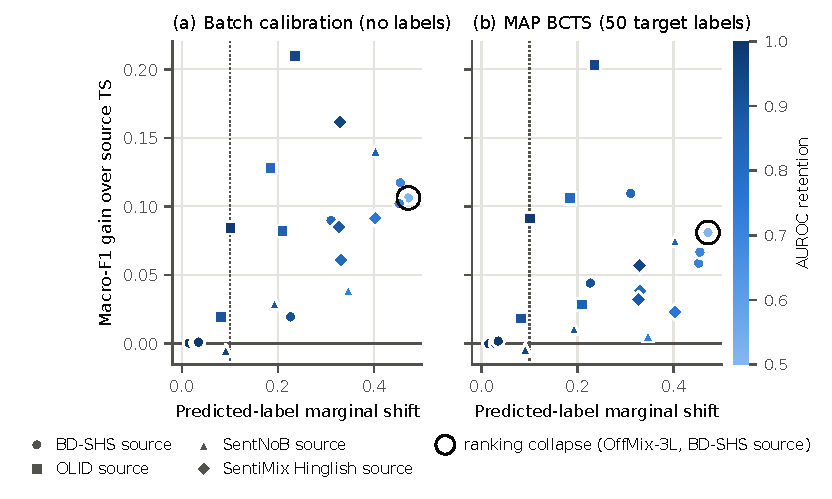
\includegraphics[width=\linewidth]{all_pairs_bias_gain.pdf}
\Description{Two scatter plots of macro-F1 gain against the shift of the predicted-label distribution for 21 source-target pairs; the gain rises with the shift for both bias corrections.}
\caption{Macro-F1 gain over source TS of a bias correction for the 21 shifted source--target pairs (means over the
converged runs of each source task). Horizontal: total-variation shift of the predicted-label distribution, computed
without target labels; dotted line at 0.10. Colour: AUROC retention. Marker shape: source task. (a) Label-free batch
calibration. (b) MAP BCTS with 50 target labels. The circled pair is the one ranking collapse.}
\label{fig:all-pairs}
\end{figure}

The descriptive regimes summarise the same picture. Encoders trained on BD-SHS keep their ranking on the Barishal and
Noakhali dialects (retention 0.994 and 0.990, marginal shift at most 0.035), and SentNoB encoders keep 0.957 of their
ranking on Sylheti; no correction improves on source TS there by more than 0.0035 nats, and spending 50 labels on the
temperature makes NLL slightly worse (0.450 against 0.442). For Sylheti this reading depends on the reference labels.
On the 72 test items on which the two authors' blind reading agreed, batch calibration raises NLL by 0.047 nats against
the SentNoB gold labels but lowers it by 0.045 against the authors' consensus, with opposite signs in every one of the
50 runs. ``No correction needed'' therefore holds against the gold labels, not against an independent reading of the
same translations. Two pairs show a finite temperature change with stable predicted proportions: the Chittagong
dialect ($\log T^{*}_{Q}/T_{P} = 0.297$, marginal shift 0.029) and BD-SHS as a target of the OLID-trained models
(0.407 and 0.082). Twelve pairs, from all four source tasks, keep a usable ranking (retention 0.70--0.98) while their
predicted marginal moves by 0.10--0.46: natural Banglish, Bangla-script code-mixing, MixTox-SA and English OLID for the
BD-SHS models; OffMix-3L, both scripts of Code-mixed Chaos and MixTox-SA for the OLID models; SentMix-3L and Hinglish
for the SentNoB models; and SentMix-3L and SentNoB for the Hinglish models. Spanglish keeps AUROC 0.609 and 0.648 for
the two sentiment sources but target TS is no better than a constant in most runs, as is Sylheti for the Hinglish
models. One pair collapses: BD-SHS models on OffMix-3L rank at AUROC 0.496 (0.387--0.589 across runs) with an
unbounded oracle temperature in every run. Where the operational thresholds are drawn moves these counts by a pair or
two (Appendix~\ref{sec:appendix-regime-sensitivity}), but not the conclusion that matters for practice: in each of the
16 pairs whose predicted marginal moves by more than 0.10, label-free bias correction raises macro-F1 in at least 93\%
of runs.

\subsection{Under a threshold shift, a temperature recovers log-loss but no decision}
\label{sec:results-threshold}

Table~\ref{tab:threshold-shift-operating-point} compares the corrections in the 12 threshold-shift pairs. Shrinkage
TS with 50 target labels lowers NLL from 0.892 to 0.728 but leaves macro-F1 at 0.527, as it must. Of the largest NLL
gain that any correction achieves, the temperature alone recovers 0.790 when units are weighted equally and 0.710 when
target corpora are: most of the log-loss, but none of the decisions. Every correction that moves the boundary changes
the decisions: batch calibration raises macro-F1 to 0.620, the MAP bias to 0.601 and MAP BCTS to 0.594, which also has
the lowest NLL among the deployable corrections (0.684). Weighting corpora equally lowers every value but keeps the
order of the methods (source TS 0.505, batch calibration 0.615, MAP BCTS 0.578); batch calibration then also has the
lower NLL (0.725 against 0.732).

\begin{table}[t]
\centering
\small
\caption{Corrections under threshold shift (R2: 12 source--target pairs, 7 target corpora, 386 run $\times$ pair units). F1 is macro-F1 on the target test split. Runs: mean over units; corpora: mean over corpora of the pair means. Labels: target labels used (50 calibration labels, 20 resamples). The last three rows are references, not deployable corrections: the true prior is the target calibration prior, the oracle bias is fitted on all target calibration labels, and the oracle threshold is tuned on the test labels themselves. Batch calibration uses the unlabelled target calibration split.}
\label{tab:threshold-shift-operating-point}
\resizebox{\textwidth}{!}{%
\begin{tabular}{lllrrrr}
\toprule
Correction & Adjusts & Labels & F1 (runs) & F1 (corpora) & NLL (runs) & NLL (corpora) \\
\midrule
Source TS & -- & 0 & 0.527 & 0.505 & 0.892 & 0.883 \\
Shrinkage TS & temperature & 50 & 0.527 & 0.505 & 0.728 & 0.771 \\
Prior adjustment, prior from labels & class prior & 50 & 0.531 & 0.524 & 0.918 & 0.882 \\
MAP bias & bias & 50 & 0.601 & 0.584 & 0.698 & 0.744 \\
MAP BCTS & temperature + bias & 50 & 0.594 & 0.578 & 0.684 & 0.732 \\
Batch calibration & bias & 0 & 0.620 & 0.615 & 0.699 & 0.725 \\
Tuned threshold & threshold & 50 & 0.631 & 0.618 & 0.713 & 0.749 \\
\midrule
Prior adjustment, true prior & class prior & prior & 0.536 & 0.531 & 0.902 & 0.864 \\
Oracle bias & bias & all & 0.626 & 0.609 & 0.665 & 0.701 \\
Oracle threshold & threshold & test & 0.660 & 0.649 & 0.693 & 0.726 \\
\bottomrule
\end{tabular}
}
\end{table}


A tuned threshold, the most direct correction of a decision, reaches 0.631 with 50 labels but has a worse NLL than the
bias corrections (0.713), and the oracle threshold tuned on the test labels themselves bounds what any correction of
this score can reach (0.660). Batch calibration is nearly as good as the NLL-optimal bias fitted on all target
calibration labels (0.620 against 0.626), so the remaining gap of the 50-label methods is an estimation problem, which
Section~\ref{sec:results-few-labels} locates. Training-time remedies that act like a temperature behave like one:
focal loss and label smoothing lower the uncalibrated ECE and NLL on most shifted conditions, but after source TS
neither is significantly better than cross-entropy on any condition, and label smoothing is significantly worse on
four of the five shifted offensive conditions (Appendix~\ref{sec:appendix-objectives}).

\subsection{The measured temperature change is mostly a misplaced bias}
\label{sec:results-decomposition}

If Proposition~\ref{prop:location} described these shifts exactly, a temperature fitted alone would rise to hedge the
misplaced threshold, while a temperature fitted jointly with a bias would stay at its source value. Fitting BCTS on all
target calibration labels of every run shows that this is what happens (Figure~\ref{fig:bcts-coordinates}). In the
threshold-shift pairs the mean change of $\log T$ is 0.976 when the temperature is fitted alone but 0.028 when it is
fitted with a bias (medians 0.989 and 0.069), and the bias alone recovers 0.932 of the BCTS log-loss gain, against
0.624 for the temperature alone. Two examples show the size of the effect: for the BD-SHS models on Bangla-script Chaos
the temperature-only change is 0.972 and the joint change $-0.075$, and for the OLID models on Banglish 1.185 and 0.078.
The temperature change survives the joint fit only where the descriptive labels say it should: on the Chittagong
dialect (0.323 alone, 0.258 jointly) and on the OffMix-3L collapse (2.461 and 2.212). The OLID models on BD-SHS, labelled
a temperature shift, sit in between (0.407 and 0.195), so part of their apparent temperature shift is also a bias.

\begin{figure}[t]
\centering
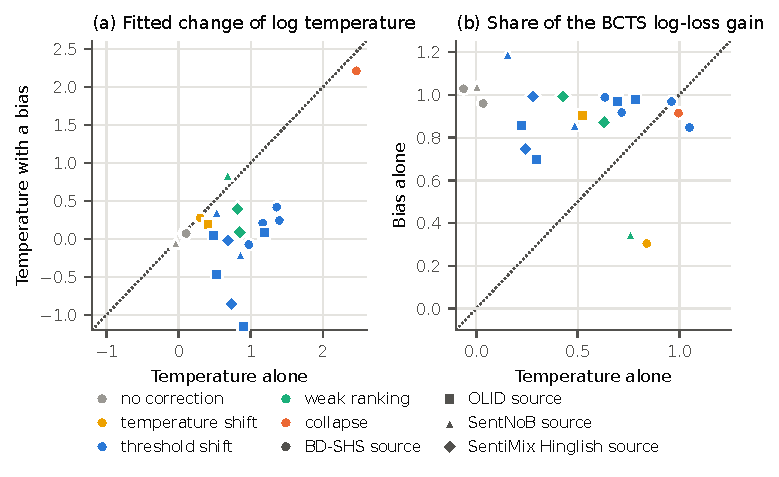
\includegraphics[width=\linewidth]{bcts_shift_coordinates.pdf}
\Description{Two scatter plots. Left: change of log temperature fitted alone against fitted jointly with a bias; threshold-shift pairs lie far below the diagonal near zero. Right: share of the log-loss gain recovered by temperature alone against bias alone; most pairs lie above the diagonal near one.}
\caption{Temperature against bias in the 21 shifted pairs (means over runs; BCTS fitted on all target calibration
labels). (a) Change of $\log T$ when the temperature is fitted alone (horizontal) and jointly with a bias (vertical);
points far below the dotted diagonal are temperature changes that a bias explains. (b) Share of the BCTS log-loss gain
recovered by the temperature alone and by the bias alone. Colour: descriptive regime; marker shape: source task.}
\label{fig:bcts-coordinates}
\end{figure}

The bias is not a change of the class prior. In the threshold-shift pairs, a prior adjustment with the true target
prior lifts macro-F1 only from 0.527 to 0.536 (Table~\ref{tab:threshold-shift-operating-point}), against 0.626 for the
oracle bias: the prior change explains almost none of the required move, and the rest is a shift of the score itself,
the $\delta$ of Proposition~\ref{prop:location}. Label-shift estimators assume that the score does not move, so they
should fail on these targets, and they do. Black-box shift estimation \citep{lipton2018bbse} and maximum-likelihood
label shift \citep{saerens2002adjusting, alexandari2020maximum} on TS and on BCTS posteriors estimate the target prior
with a total-variation error of 0.297--0.480 on the five BD-SHS-source targets beyond the dialects, whose true prior
moves by only 0.001--0.149 from the source, and they lower macro-F1 below source TS on every pair whose predicted
marginal moves by more than 0.10. On Banglish, for instance, macro-F1 falls from 0.577 to 0.450, 0.411 and 0.392, while
batch calibration reaches 0.666. Even where the prior really changes, for OLID models on BD-SHS (total variation
0.149), none of the three estimators recovers it (errors 0.153, 0.220 and 0.187), whereas the true prior would raise
macro-F1 from 0.681 to 0.699. The failure of these estimators is a symptom: the label-shift assumption does not hold
for dialect, script and code-mixing shift.

\subsection{What 50 labels can and cannot fix}
\label{sec:results-few-labels}

MAP BCTS trails batch calibration in macro-F1 although it uses labels. Projecting the bias that each method fits from
50 labels onto the oracle bias, with 1 meaning the full move, locates the shortfall. On the offensive targets the
maximum-likelihood bias reaches a median of 0.960 of the move and the MAP bias 0.873; on the sentiment targets the
maximum-likelihood bias reaches 0.980 but the MAP bias only 0.314 and the bias of MAP BCTS 0.187, against 0.639 for the
bias implied by batch calibration. The sentiment prior variance for the bias is estimated from the offensive task and
is small, so it holds the sentiment bias near its source value. The labels are informative; the prior, not the label
budget, is why MAP BCTS falls behind on the threshold-shift pairs.

Batch calibration has its own assumption: it pulls the predicted proportions towards uniform. Resampling every target
of the two offensive source tasks to a fixed positive share $\pi_+$ shows when this backfires
(Table~\ref{tab:prior-shift-ablation} in the appendix). At $\pi_+ = 0.1$, the typical situation in content moderation,
batch calibration lowers macro-F1 to 0.631 from 0.654 with source TS and raises NLL from 0.31 to 0.56; a class prior
estimated from 50 labels repairs the rare-positive case on average (0.661 and 0.27), as does MAP BCTS (0.665 and
0.25), although both stay worse than source TS in 30\% and 46\% of units on macro-F1. Every correction fitted on
target items also inherits their prior. When the 50 labels and the unlabelled batch come from a target with
$\pi_+ = 0.9$ and the deployment stream has $\pi_+ = 0.1$, MAP BCTS falls to macro-F1 0.252 and is better than source
TS (0.651) in none of the units, the label-estimated prior reaches 0.421, and batch calibration, whose uniform target
does not depend on the batch prior, reaches 0.680. In the reverse direction (0.1 to 0.9) the four give 0.434, 0.359,
0.404 and 0.575 in the same order of source TS, MAP BCTS, label-estimated prior and batch calibration. With matched
priors at 0.5 MAP BCTS is the best of them (0.713). The few-label recipe therefore assumes that the labelled items come
from the deployment distribution, and a correction must be refitted when the prior drifts.

\subsection{Robustness}
\label{sec:results-robustness}

The 12 threshold-shift pairs rest on seven target corpora. In every one of them batch calibration raises the mean
macro-F1 (exact two-sided sign test, 7 of 7, $p = 0.0156$), and the same holds for the nine corpora of the 16 pairs
with a predicted-marginal shift above 0.10 (9 of 9, $p = 0.0039$). Without the two student-written corpora, OffMix-3L
and SentMix-3L, five corpora remain and five of five are positive, which gives $p = 0.0625$, the smallest value a
two-sided sign test can reach with five units; the corpus-weighted gain is 0.081 with a hierarchical bootstrap 95\%
interval of 0.052--0.105. On the natural corpora of the pairs with a marginal shift above 0.10, 7 of 7 are positive
($p = 0.0156$; gain 0.076, interval 0.055--0.096). A mixed model with random intercepts for corpus and for pair within
corpus gives a threshold-shift gain of 0.108 (standard error 0.020, $z = 5.38$, 95\% interval 0.069--0.147) and, over
all 21 pairs, a slope of 0.219 on the predicted-marginal shift ($z = 2.31$, $p = 0.021$;
Appendix~\ref{sec:appendix-mixed}). Seven purposively chosen corpora cannot support a claim about a population of
corpora; these checks show that the effect is not carried by one corpus or one weighting.

\section{Script, Source Corpus and the One Collapse}
\label{sec:results-interventions}

The diagnosis so far took each model's scores as given. Two interventions now ask what moves them while holding the
target items fixed: the first changes only the script in which the target comments are written, the second changes
the corpus on which the model was trained.

\subsection{The same comments in another script}
\label{sec:results-script}

Code-mixed Chaos comes in Banglish and in a row-aligned Bangla-script rendition of the same comments with identical
labels. The release describes this rendition as a transliteration and also as a translation, so the comparison holds
the comments and labels fixed but may change some wording along with the script. Moving the comments into Bangla
script raises encoder AUROC by 0.212--0.225 for IndicBERT (four training variants), 0.159 for mDeBERTa-v3,
0.071--0.096 for XLM-R-base, 0.043 for MuRIL and 0.022--0.036 for BanglaBERT, while the zero-shot language models
change by $-0.001$ to $+0.055$ (Figure~\ref{fig:script}). Script coverage thus explains part of the encoders'
difficulty with romanised text, and most for the models whose pretraining saw least of it. It also moves the
threshold: the BD-SHS encoders label 16.4\% of the Banglish comments as toxic and 26.1\% of the same comments in Bangla
script, against 50\% in the gold labels, so even with the script restored the predicted proportions remain far from
the target's. Script coverage does not explain the OffMix-3L collapse: MuRIL, which was pretrained with
transliterated text, still ranks OffMix-3L at 0.546.

\begin{figure}[t]
\centering
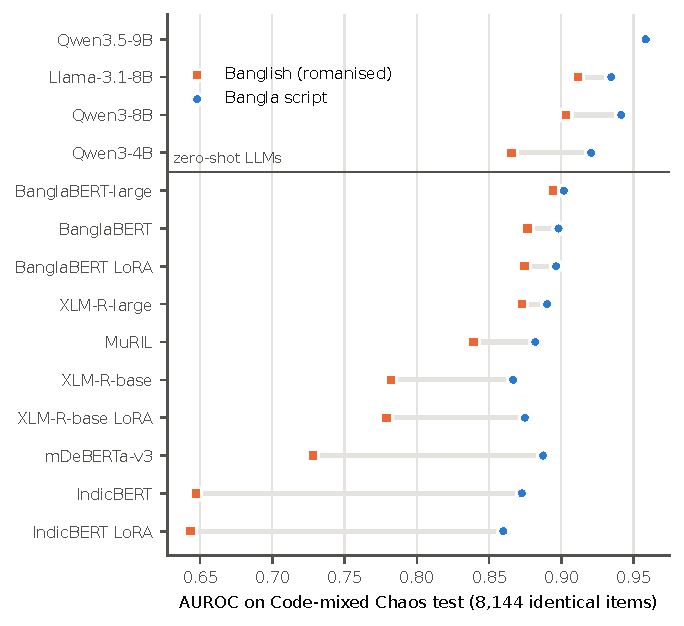
\includegraphics[width=\linewidth]{script_intervention_auroc.pdf}
\Description{Dot plot of AUROC for each encoder configuration and language model on the same comments in Banglish and in Bangla script; encoders gain up to about 0.2 from the Bangla script, language models change little.}
\caption{The same Code-mixed Chaos test comments in Banglish and in Bangla script: AUROC of every BD-SHS-trained
encoder configuration (mean over converged runs) and of each zero-shot language model, after each system's source
TS.}
\label{fig:script}
\end{figure}

\subsection{Changing the source corpus: a definition-by-language factorial}
\label{sec:results-factorial}

BD-SHS annotates hate speech \citep{romim2022bdshs}. OffMix-3L shares the label set of OLID, whose guidelines count
any unacceptable language as offensive, including untargeted profanity \citep{zampieri2019olid}, and its authors
build their synthetic training data from English corpora with those labels \citep{goswami2023offmix}. Training the
same three architectures on English OLID instead of BD-SHS raises OffMix-3L AUROC from 0.519 to 0.819, but this
comparison changes the training corpus, its label definition and its language at once. The factorial separates the
language. Cells A and B are the untranslated sources (BD-SHS in Bangla, OLID in English); C is OLID translated into
Bangla and D is BD-SHS translated into English; E and F are round trips that bring each corpus back to its own language
through the other one. Within each language two machine-translated cells then differ in their source corpus (E
against D in English, C against F in Bangla), and also in the number of translation passes (two for E and F, one for C
and D); the main effect over the four translated cells balances the passes.

\begin{figure}[t]
\centering
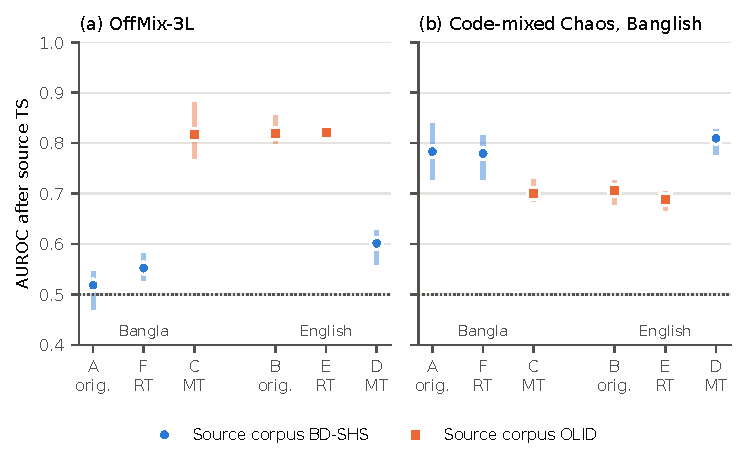
\includegraphics[width=\linewidth]{source_corpus_factorial.pdf}
\Description{Two panels of AUROC for six training cells; on OffMix-3L the OLID-based cells rank near 0.82 and the BD-SHS-based cells between 0.52 and 0.60, while on Banglish the order reverses.}
\caption{AUROC of the six factorial cells after source TS: XLM-R-base, MuRIL and mDeBERTa-v3 trained on each source
(points: mean over the 15 runs; bars: range of the three architecture means). Bangla cells: A, BD-SHS; F, BD-SHS after
a round trip through English; C, OLID translated into Bangla. English cells: B, OLID; E, OLID after a round trip
through Bangla; D, BD-SHS translated into English. orig.: untranslated; MT: translated; RT: round trip.}
\label{fig:factorial}
\end{figure}

The family of four contrasts on OffMix-3L AUROC was fixed in the public repository before cells C to F were trained
but after A and B were known, so it is pre-specified for the translated cells rather than for the whole experiment. All four favour the OLID corpus (Figure~\ref{fig:factorial}): $+0.220$ in English (E minus D, 95\%
interval 0.175--0.267), $+0.264$ in Bangla (C minus F, 0.207--0.316), $+0.242$ for the main effect over the four
translated cells (0.205--0.278), and $+0.343$ for its difference-in-differences against Banglish Chaos (0.311--0.375),
each with a Holm-adjusted stratified permutation $p < 0.001$ over 15 runs per cell. The language of the translated
training data matters far less: the language main effect on OffMix-3L is $-0.027$ (interval $-0.059$ to $0.006$,
$p = 0.132$). Within five writing-style clusters of OffMix-3L, which absorb much of its artifacts, the source-corpus
effect remains ($+0.209$ in English and $+0.244$ in Bangla).

The same contrast does not generalise. On natural Banglish the source-corpus main effect reverses to $-0.101$
(interval $-0.112$ to $-0.089$), on the BD-SHS test set it is $-0.129$, and on the OLID test set $+0.101$: each corpus
ranks its own kind of text best, and on MixTox-SA the effect is $-0.005$ ($p = 0.431$). The factor that the factorial
manipulates is therefore the source corpus together with its translation pipeline, that is, its label definition,
annotators and sampling of text as they survive machine translation, rather than the definition alone, and the inference covers the variation over seeds and architectures given one
translation, one MT system and one target. Translation also removes offensive words more than other words: over a
round trip, OLID keeps 0.680 of the offensive-associated words of offensive items (95\% interval 0.625--0.733) against
0.817 for frequency-matched control words, and BD-SHS keeps 0.249 against 0.294. This word-level sanitisation is a
limitation of the translated cells, but it cannot produce the OffMix-3L result, since the OLID-based cells that lost
those words still rank OffMix-3L at 0.816 and 0.822. We read the OffMix-3L collapse as a mismatch between the BD-SHS
corpus and that target, a property of a student-written stress case rather than of code-mixing; the natural
code-mixed targets, on which BD-SHS models keep their ranking, carry the general claims. Matching the corpus restores
the ranking but not the threshold: the OLID-trained models label 8.4\% of OffMix-3L as offensive, against 47.8\% in the
gold labels, which is the threshold shift of Section~\ref{sec:results-diagnosis} again.

\section{Label-Efficient Shift Triage}
\label{sec:shift-triage}
[Draft pending.]

\section{Related Work}
\label{sec:related-work}

\paragraph{Calibration under distribution shift.}
Modern networks are overconfident, and temperature scaling is a strong post-hoc repair in domain
\citep{guo2017calibration}; calibration degrades under dataset shift \citep{ovadia2019trust}. For pre-trained
transformers, \citet{desai2020calibration} found temperature scaling effective in and out of domain on English tasks,
\citet{kong2020calibrated} regularise fine-tuning for calibration in and out of distribution,
\citet{ahuja2022multilingual} report miscalibration of multilingual models under cross-lingual transfer, and
\citet{yang2026multilingualqa} study multilingual question answering; \citet{roschewitz2025where} give the image-classification
counterpart of a large calibration study under dataset shift. We decompose
the failure into temperature, threshold and ranking components and show that, under language-variety shift, the
threshold component dominates and is invisible to temperature-only methods.

\paragraph{Label shift and bias correction.}
Prior adjustment by EM \citep{saerens2002adjusting}, black-box and related shift estimators
\citep{lipton2018bbse, garg2020unified} and
bias-corrected calibration \citep{alexandari2020maximum} address a change of the class prior with fixed class-conditional
distributions, and posterior recalibration interpolates towards a target prior \citep{tian2020posterior}. For prompted
LLMs, contextual calibration \citep{zhao2021calibrate} and batch calibration \citep{zhou2024batch} estimate a bias
without labels. Our targets violate the label-shift assumption: in four threshold-shift pairs the predicted proportions move while
the true ones barely do, and EM prior estimation lowers macro-F1 on every code-mixed and cross-language target
(Appendix~\ref{sec:appendix-recalibration}). We find that a
bias correction is nevertheless the right repair, that its label-free form backfires when positives are rare, and that
a prior from 50 labels repairs it on average.

\paragraph{Conformal prediction and risk control.}
Split conformal prediction and conformal risk control give finite-sample guarantees under exchangeability
\citep{angelopoulos2024crc}, and can be reweighted for a known label shift \citep{podkopaev2021distribution}. Weighted conformal prediction handles covariate shift with known density ratios
\citep{tibshirani2019weighted}; our source and target barely overlap, so there is little to reweight. Choosing among models with the same calibration data breaks the
guarantee unless corrected \citep{liang2024conformal}; we use Bonferroni and sample-splitting corrections and report
their cost.

\paragraph{Code-mixing, dialects and cross-dataset offensive-language detection.}
Code-mixed benchmarks \citep{khanuja2020gluecos, aguilar2020lince, patwa2020sentimix, goswami2023offmix} and
dialect transformations \citep{ziems2023multivalue} document accuracy drops on mixed-language and dialectal text, and hate-speech detectors are known to generalise poorly across datasets, in part
because their definitions differ \citep{yin2021generalisable, fortuna2021generalize}. Our interventions point to such a
definition mismatch as the likely source of the only ranking collapse in our study; the far more common failure is one
of calibration that the ranking survives.

\section{Discussion and Limitations}
\label{sec:discussion}

\paragraph{What to do in practice.}
Detect shift with a domain classifier, not with the model's confidence. After a detected shift, correct the class bias
rather than only the temperature. Without labels, batch calibration is the strongest single correction on
near-balanced targets, but it should not be used when positives may be rare. With about 50 labels drawn from the
deployment stream, estimate the prior or fit the bias, choose between the fine-tuned encoder and a language model, and
refit whenever the class prior of the stream may have drifted, because every correction fitted on target items
inherits their prior. On a near-balanced target the same labels test a strong ranking and certify coverage; on a skewed
target the false-negative certificate needs 19 labelled positives, hence hundreds of random labels. Fine-tuning on the
target becomes the better use of labels only at a few hundred labels.

\paragraph{Why thresholds move.}
The decomposition of Section~\ref{sec:results-decomposition} says where the move comes from: the scores of the target
items shift relative to the source, mostly for both classes alike, and little of the move is a change of the class
prior. It does not say why the scores shift. One account consistent with the script intervention is that text the
encoder reads poorly receives scores close to those of bland in-domain text, which pushes its predictions towards the
non-offensive class; restoring the script raises the predicted toxic share but leaves it far below the target's.
Testing this account would need targets whose readability for the encoder can be varied while the content stays fixed,
which the two scripts of Code-mixed Chaos provide only for one pair of conditions.

\paragraph{Limitations.}
The study covers two classification tasks. The main grid is Bangla, and the English and Hindi--English sources use
three architectures each, against seven for the Bangla sources; encoders have up to 560M parameters and language
models up to 9B, and generative tasks and proprietary models are not covered. The 21 pairs come from 11 purposively
chosen corpora and the 12 threshold-shift pairs from seven, so the results describe these corpora rather than a
population of shifts, and two of the seven corpora are student-written; the corpus-level tests of
Section~\ref{sec:results-robustness} show how far the effect holds without them. The regime labels and their thresholds
were set after the results had been seen, and we state the practical conclusions over all pairs instead.

Several limitations concern the data. The Sylheti set is small and was translated by two of the authors, and whether a
correction helps on it depends on whether the gold or the authors' consensus labels are the reference. OffMix-3L
carries strong writing-style artifacts and labels that two readers could not reproduce, so it serves only as a stress
case. Most targets are close to balanced, which favours label-free batch calibration, and the few-label results assume
that the labelled items come from the deployment distribution; under prior drift MAP BCTS can fall far below source TS.
The Spanglish calibration and test splits come from different releases. The language-model prompt describes Hinglish
and Spanglish text as Bangla; a language-neutral prompt did not change the result, but the main comparison uses the
original prompt.

The factorial isolates the source corpus rather than the label definition: each translated cell comes from one MT
system and one translation, its inference covers seeds and architectures only, and translation removes
offensive-associated words more than other words. The distance-aware calibrator is adapted to a reference bank drawn
from the source calibration split, because training-split representations were not stored. Many results are
descriptive means over runs; formal tests with multiplicity control are reported for the families fixed in the code,
and five-versus-five comparisons cannot reach significance after correction in large families. The guarantees of
Section~\ref{sec:shift-triage} are marginal over target calibration and test items and assume exchangeability within
the target. Finally, no item-level memorisation by the language models was detected, but exposure to the public test
sets cannot be excluded.

\section{Conclusion}
\label{sec:conclusion}

Across the dialects, scripts, code-mixing and languages we studied, on two tasks centred on Bangla and with source tasks
in three languages, the common failure of the fine-tuned classifiers was a misplaced decision threshold, not a wrong
temperature.
Temperature scaling cannot move the threshold however many labels it is fitted on; a bias correction can, provided its
assumption about the class prior is checked with a few labels. A collapse of the ranking is rare, appears here to
arise from a mismatch of label definitions, and no post-hoc map repairs it.


\section*{Broader Impact Statement}
[Draft pending.]


\bibliographystyle{ACM-Reference-Format}
\bibliography{references}

\appendix
\section{Additional Results}
\label{sec:appendix-results}
[Draft pending.]


\end{document}
